\documentclass[12pt, psamsfonts]{amsart}

%-------Packages---------
\usepackage{listings}
\usepackage{semantic}
\usepackage{breqn}
\usepackage{amssymb,amsfonts}
\usepackage{fullpage}
\usepackage{tikz-cd}
\usepackage{todonotes}
\usepackage{physics}
\usepackage[all,arc]{xy}
\usepackage{enumerate}
\usepackage{enumitem}
\usepackage{mathrsfs}
\usepackage{theoremref}
\usepackage{graphicx}
\usepackage[bookmarks]{hyperref}

%--------Theorem Environments--------
%theoremstyle{plain} --- default
\newtheorem{thm}{Theorem}[section]
\newtheorem{cor}[thm]{Corollary}
\newtheorem{prop}[thm]{Proposition}
\newtheorem{lem}[thm]{Lemma}
\newtheorem{conj}[thm]{Conjecture}
\newtheorem{quest}[thm]{Question}

\theoremstyle{definition}
\newtheorem{defn}[thm]{Definition}
\newtheorem{defns}[thm]{Definitions}
\newtheorem{con}[thm]{Construction}
\newtheorem{exmp}[thm]{Example}
\newtheorem{exmps}[thm]{Examples}
\newtheorem{notn}[thm]{Notation}
\newtheorem{notns}[thm]{Notations}
\newtheorem{addm}[thm]{Addendum}
\newtheorem*{exer}{Exercise}

\theoremstyle{remark}
\newtheorem{rem}[thm]{Remark}
\newtheorem{rems}[thm]{Remarks}
\newtheorem{warn}[thm]{Warning}
\newtheorem{sch}[thm]{Scholium}

\DeclareMathOperator{\Hom}{Hom}
\DeclareMathOperator{\Id}{Id}
\DeclareMathOperator{\End}{End}
\DeclareMathOperator{\ord}{ord}
\DeclareMathOperator{\Aut}{Aut}
\DeclareMathOperator{\Gal}{Gal}

\makeatletter
\let\c@equation\c@thm
\makeatother
\numberwithin{equation}{section}

\bibliographystyle{plain}

\begin{document}

\title{Math 601 (Due 11/22)}
\author{Hidenori Shinohara}
\maketitle

\tableofcontents
\section{The Theorem on Symmetric Polynomials}

\begin{exer}{(Problem 1)}
  By substituting $u_4 = 0$, we get $u_1^2u_2u_3 + u_1u_2^2u_3 + u_1u_2u_3^2 = s_3s_1$.
  $s_3s_1$ with 4 variables expands to $u_{1}^{2} u_{2} u_{3} + u_{1}^{2} u_{2} u_{4} + u_{1}^{2} u_{3} u_{4} + u_{1} u_{2}^{2} u_{3} + u_{1} u_{2}^{2} u_{4} + u_{1} u_{2} u_{3}^{2} + 4 u_{1} u_{2} u_{3} u_{4} + u_{1} u_{2} u_{4}^{2} + u_{1} u_{3}^{2} u_{4} + u_{1} u_{3} u_{4}^{2} + u_{2}^{2} u_{3} u_{4} + u_{2} u_{3}^{2} u_{4} + u_{2} u_{3} u_{4}^{2}$.
  Then $s_3s_1 - f$ where $f$ is the original polynomial gives us $4u_1u_2u_3u_4 = 4s_4$.
  Therefore, $f = s_3s_1 - 4s_4$.
\end{exer}

\begin{exer}{(Problem 2)}
  We are given that $\abs{xI - M} = x^3 - ax^2 + bx - c$.
  This implies that $\abs{(-xI) - M} = -x^3 - ax^2 - bx - c$.
  Since the determinant function preserves multiplication, $\abs{xI - M}\abs{-xI - M} = \abs{M^2 - x^2I}$.
  This implies $\abs{M^2 - x^2I} = -x^6 + (a^2 - 2b)x^4 + (-b^2 + 2ac)x^2 + c^2$.
  Therefore, $\abs{yI - M^2} = y^3 + (2b - a^2)y^2 + (b^2 - 2ac)y - c^2$.
\end{exer}

\section{Galois Theory VI}

\begin{exer}{(Problem 3)}
  \begin{enumerate}[label=(\roman*)]
    \item
      $\{ (123), (132), e \}$ is clearly a subgroup of the stabilizer group $S_v$ of $v$.
      Since $(12) \notin S_v$, $3 \leq \abs{S_v} \leq 5$.
      By Lagrange's Theorem, $S_v = \ev{(123)}$. 
    \item
      By (i), $S_3v$ contains only $[S_3:S_v] = 2$ elements.
      Thus $v' = (12) \cdot v = u_2u_1^2 + u_1u_3^2 + u_3u_2^2$.
    \item
      By substituting $u_3 = 0$ for $v + v'$, we get $u_1u_2^2 + u_2u_1^2 = s_1s_2$.
      Then $v + v' - s_1s_2 = -3u_1u_2u_3 = -3s_3$.
      Therefore, $v + v' = s_1s_2 - 3s_3$.
    \item
      We will use the fundamental theorem of Galois Theory.
      $F(v) = K^{\ev{(123)}}$, so $\abs{\ev{(123)}} = 3 = [K:F(v)]$.
      Moreover, $\abs{\ev{\Gal(K/F)}} = [K:F]$.
      Therefore, $[F(v):F] = [K:F]/[K:F(v)] = \abs{\Gal(K/F)}/3$.
    \item
      Calculation shows that $vv' = 9s_3^2 + s_3s_1^3 - 6s_3s_1s_2 + s_2^3$.
      By substituting $s_1 = 0, s_2 = p, s_3 = q$, we get $9q^2 + p^3$.
    \item
      Since $A_3$ is the only proper transitive subgroup of $S_3$, $\Gal(K/F) = S_3$ if and only if $\sigma \in \Gal(K/F)$ where $\sigma$ corresponds to the permutation $(12)$.
      (i.e., $u_1 \mapsto u_2, u_2 \mapsto u_1$.)
      $v, v'$ are not fixed by $\sigma$, so $v, v' \notin F$ if $\Gal(K/F) = S_3$.
      $v, v'$ are fixed by every permutation if $\Gal(K/F) = A_3$ because it is generated by $\sigma'$ that corresponds to $(123)$.
      Therefore, we can conclude that $\Gal(K/F) \ne S_3$ if and only if $v, v' \in F$.
      $v, v' \in F$ if and only if $(y - v)(y - v')$ factors in $F$.
      Therefore, $h(y) = y^2 - (v + v')y + vv' = y^2 + 3qy + (9q^2 + p^3)$ is the desired polynomial.
    \item
      The discriminant is $(3q)^2 - 4(9q^2 + p^3) = 9q^2 - 36q^2 - 4p^3 = -27q^2 - 4p^3$.
  \end{enumerate}
\end{exer}

\begin{exer}{(Problem 4)}
  \begin{enumerate}[label=(\roman*)]
    \item 
      The discriminant can be expressed as $-4s_{1}^{3}s_{3}+s_{1}^{2}s_{2}^{2}+18s_{1}s_{2}s_{3}-4s_{2}^{3}-27s_{3}^{2}$.
      By substituting $s_1 = 1, s_2 = -2, s_3 = -1$, we get 49.
      \mathligsoff
      \lstinputlisting[language=python]{galois_problem4.py}
      \mathligson
      Since the discriminant is a square, the Galois group is isomorphic to $A_3$.
    \item
      Since $\Gal(K/\mathbb{Q}) = A_3$, the degree of extension is 3.
      First, we claim that $K \subset \mathbb{R}$.
      If $K$ is not a subset of $\mathbb{R}$, $\sigma(a + bi) = a - bi \in \Gal(K/\mathbb{Q})$.
      However, this is impossible because $\abs{\sigma} = 2 \nmid 3 = \abs{A_3}$.

      Let $\sigma \in \Gal(K/\mathbb{Q})$ be given.
      Since the degree of extension is 3, there cannot be any intermediate field.
      Therefore, if $a^{1/n} \notin \mathbb{Q}$, $\mathbb{Q}(a^{1/n}) = K$.
      Hence, we can uniquely determine $\sigma$ by checking $\sigma(a^{1/n})$.
      Since $a^{1/n}$ is a root of $x^n - a$, $\sigma(a^{1/n})$ must be a root of $x^n - a$.
      Since $K \subset \mathbb{R}$, $\sigma(a^{1/n}) = \pm a^{1/n}$.
      It is impossible that $\sigma(a^{1/n}) = -a^{1/n}$ since this implies $\abs{\sigma} = 2 \nmid 3$.
      Therefore, $\sigma = \Id$, but this implies that $\Gal(K/\mathbb{Q})$ is trivial, which is a contradiction.

      Thus $a^{1/n} \in \mathbb{Q}$.
  \end{enumerate}
\end{exer}

\begin{exer}{(Problem 5)}
  \begin{enumerate}[label=(\roman*)]
    \item 
      By modifying the code for Problem 4, we obtain that
      \begin{align*}
        &-27s_{1}^{4}s_{4}^{2}+18s_{1}^{3}s_{2}s_{3}s_{4}-4s_{1}^{3}s_{3}^{3}-4s_{1}^{2}s_{2}^{3}s_{4}+\\
        &s_{1}^{2}s_{2}^{2}s_{3}^{2}+144s_{1}^{2}s_{2}s_{4}^{2}-6s_{1}^{2}s_{3}^{2}s_{4}-80s_{1}s_{2}^{2}s_{3}s_{4}+\\
        &18s_{1}s_{2}s_{3}^{3}-192s_{1}s_{3}s_{4}^{2}+16s_{2}^{4}s_{4}-4s_{2}^{3}s_{3}^{2}-128s_{2}^{2}s_{4}^{2}+\\
        &144s_{2}s_{3}^{2}s_{4}-27s_{3}^{4}+256s_{4}^{3}
      \end{align*}
      We are given that $s_1 = s_2 = 0$.
      Therefore, we are left with $256s_4^3 - 27s_3^4 = 256b^3 - 27a^4$.
    \item
      $x^4 + x + 1$ is irreducible because
      \begin{itemize}
        \item
          It does not have a linear factor by the rational root theorem.
        \item
          If it factors into two rational quadratic polynomials, they will factor into two monic integer quadratic polynomials, namely, $x^2 + ax + b$ and $x^2 - ax + 1/b$ based on the coefficients.
          This implies $b = \pm 1$.
          Since the coefficient of x is 1, $-ab + a/b = 1$, but this implies $b \ne \pm 1$.
      \end{itemize}
      We will use the discussion presented in the Galois Theory IV handout.
      By (i), the discriminant is 229, so $h(y) = y^2 - 229$.
      Also, $g(y) = y^3 - 4y - 1$ since $a = b = 0, c = -1, d = 1$.
      Therefore, both $h(y)$ and $g(y)$ are irreducible, so the Galois group is $S_4$.
    \item
      It does not have a linear factor by the rational root theorem.
      Based on coefficients, if it factors into quadratic polynomials, it will be $(x^2 + ax + b)(x^2 - ax + c)$ for some $a, b, c \in \mathbb{Z}$ by Gauss' lemma.
      This gives $bc = 12$ and $-ab + ac = -8$, so $a(c - 12/c) = -8$.
      This is a quadratic polynomial in $c$ with the discriminant $64 - 48a$.
      This must be a square for $c$ to exist.
      By checking each possible value of $a$, we get $64 - 48 \cdot -8 = 448, 64 - 48 \cdot -4 = 256, 64 - 48 \cdot -2 = 160, 64 - 48 \cdot -1 = 112, 64 - 48 \cdot 1 = 16$.
      (For other $a$, $64 - 48a < 0$.)
      Thus the only two possible values are $a = 1, -4$.
      $a = 1$ gives $c - b = -8$ and $bc = 12$, which we can confirm to be impossible by examining the divisors of 12.
      Similarly, $a = -4$ gives $c - b = 2$ and $bc = 12$ and this is impossible to satisfy.
      Therefore, $x^4 - 8x + 12$ is irreducible over $\mathbb{Q}$.
    \item
      Again, we will use the discussion presented in the Galois Theory IV handout.
      By calculating the discriminant, we have $h(y) = h(y) = y^{2} - 331776$ and $g(y) = y^{3} - 48 y - 64$.
      $h(y)$ factors as $576^2 = 331776$.
      $g(y)$ does not factor by the rational root theorem.
      Therefore, the Galois group is $A_4$.
  \end{enumerate}
\end{exer}

\section{Galois Theory V(Further exercises)}

\begin{exer}{(Problem 3)}
  \begin{enumerate}[label=(\roman*)]
    \item 
      $x^n - 1$ cannot split in a field smaller than $K$ because $\zeta$ is a root.
      On the other hand, $\{ \zeta^i \mid 0 \leq i \leq n - 1 \}$ contains $n$ distinct roots of $x^n - 1$.
      Therefore, $K$ is the splitting field of $x^n - 1$.
    \item
      $\phi(n)$ because for any $1 \leq m \leq n - 1$ such that $d = \gcd(m, n) \ne 1$, $(\zeta^m)^d = 1$, so $\zeta^m$ is not a primitive $n$th root.
      On the other hand, $(\zeta^m)^k = 1$ with $1 \leq k \leq n - 1$, then $n \mid mk$, so $\gcd(n, m) \ne 1$.
    \item
      All the primitive roots are roots of $x^n - 1$.
      Since $\sigma \in \Aut(K/F)$ permutes the roots of $x^n - 1$, all the primitive roots get mapped to roots of $x^n - 1$.
      Suppose that $\sigma(\zeta) = \zeta'$ where $\zeta'$ is not a primitive root.
      Then $\zeta'$ satisfies $x^m - 1$ where $m < n$.
      This implies that $\sigma^{-1}$ sends $\zeta'$, a root of $x^m - 1$, to $\zeta$, which is not a root of $x^m - 1$.
      This is a contradiction, so all the primitive roots must get mapped to primitive roots.

      Therefore, any automorphism in $\Aut(K/F)$ sends primitive roots to primitive roots.
    \item
      $\abs{(\mathbb{Z}/n)^*} = \phi(n)$ where $\phi(n)$ is Euler's totient function.
    \item
      $a \mapsto \zeta^a$.
    \item
      Let $\Phi: \Aut(K/F) \rightarrow (\mathbb{Z}/n)^*$ be defined such that $\Phi(\sigma) = m$ where $\sigma(\zeta) = \zeta^m$.
      \begin{itemize}
        \item
          Well-defined?
          Every automorphism in $\Aut(K/F)$ sends a primitive $n$th root to a primitive $n$th root as shown in (iii).
          Therefore, $m$ must be coprime to $n$, so $\Phi(\sigma) \in (\mathbb{Z}/n)^*$ for all $\sigma \in \Aut(K/F)$.
        \item
          Group homomorphism?
          Let $\sigma_1, \sigma_2 \in \Aut(K/F)$ be given.
          Let $m_1, m_2$ be chosen such that $\sigma_1(\zeta) = \zeta^{m_1}, \sigma_2(\zeta) = \zeta^{m_2}$.
          Then $\sigma_1 \circ \sigma_2$ maps $\zeta$ to $\zeta^{m_1m_2}$.
          Therefore, $\Phi(\sigma_1 \circ \sigma_2) = m_1m_2 = \Phi(\sigma_1)\Phi(\sigma_2)$.
        \item
          Injective?
          It suffices to check $\ker(\Phi)$.
          If $\sigma \in \ker(\Phi)$, then $\sigma(\zeta) = \zeta^1$, so $\sigma = \Id$.
          Thus the kernel is trivial.
      \end{itemize}
      Therefore, $\Phi$ is a well-defined, injective group homomorphism.
    \item
      We showed earlier that $\{ \zeta^0, \zeta^1, \cdots, \zeta^{n - 1} \}$ are the $n$ distinct roots of $x^n - 1$.
      Thus $x^n - 1$ is separable.
      By Theorem 8 of the Galois Theory II handout, $\Aut(K/F) = [K:F]$
      Therefore, this is a Galois extension.
      Moreover, $\Aut(K/F)$ can be embedded in $(\mathb{Z}/n)^*$, which is clearly an abelian group.
      Therefore, $\Aut(K/F)$ is abelian.
    \item
      Let $\zeta = e^{2\pi i/5}$ and $K = \mathbb{Q}(\zeta)$.
      Then $\zeta$ is a primitive 5th root.
      $x^5 - 1 = (x - 1)(x^4 + x^3 + x^2 + x + 1)$.
      Thus $\zeta$ is a root of $f(x) = x^4 + x^3 + x^2 + x + 1$.
      By substituting $x = x + 1$, we obtain $x^4 + 5x^3 + 10x^2 + 10x + 5$, which is irreducible by Eisenstein.
      Therefore, $f(x)$ must be irreducible.

      By the argument above, $\Aut(K/F)$ can be embedded in $(\mathbb{Z}/5)^* = \ev{2}$.
      This implies that $\Aut(K/F)$ either contains 1, 2, 4 elements.
      Since $\Aut(K/F)$ has to be transitive, it cannot be trivial.
      Suppose $\Aut(K/F)$ has two elements.
      Let $r_1, \cdots, r_4$ denote the 4 distinct roots of $x^4 + x^3 + x^2 + x + 1$.
      There must be a $\sigma \in \Aut(K/F)$ such that $r_2 = \sigma(r_1)$.
      However, $\sigma$ must be the only nontrivial element in $\Aut(K/F)$.
      Then there is no automorphism in $\Aut(K/F)$ that sends $r_1$ to $r_3$.
      Therefore, $\Aut(K/F)$ is not transitive if it only contains two elements.

      Therefore, $\Aut(K/F)$ must contain 4 elements, and thus $\Aut(K/F) \cong (\mathbb{Z}/5)^* = \ev{2}$.
  \end{enumerate}
\end{exer}
\section{Galois Theory V}

\begin{exer}{(Problem 1)}
  \begin{enumerate}[label=(\roman*)]
    \item 
      $D_4$ is a subgroup of $S_4$ and the Galois Theory V handout states that $S_4$ is solvable and any subgroup of a finite solvable group is solvable.
    \item
      If $S_5$ is solvable, $A_5 \leq S_5$ is solvable.
      However, as stated in the handout, $A_5$ is not solvable.
  \end{enumerate}
\end{exer}

\begin{exer}{(Problem 2)}
  \begin{enumerate}[label=(\roman*)]
    \item 
      Let $a = (12345)$ and $b = (2354)$.
      Since $\abs{a} = 5$ and $\abs{b} = 4$, $20 \mid \abs{G}$.
      On the other hand, every element can be written as $a^ib^j$ because of the relation $ab = (1243) = ba^3$.
      Since every element can be written as $a^ib^j$ where $0 \leq i \leq 4$ and $0 \leq j \leq 3$, $G$ contains exactly 20 elements.
    \item
      $G$ has a subgroup $G_1 = \{(1),$ $(12)(35),$ $(12345),$ $(13)(45),$ $(13524),$ $(14)(23),$ $(14253),$ $(15)(24),$ $(15432),$ $(25)(34)\}$.
      of index 2.
      $G_1$ has a subgroup $G_2 = \{(1),$ $(12345),$ $(13524),$ $(14253),$ $(15432)\}$ of index 2.
      $G_2$ is abelian, so we can pick $G_3 = \{(1)\}$.
      Then $G_3 \subset G_2 \subset G_1 \subset G$ is a filteration. 
  \end{enumerate}
\end{exer}

\begin{exer}{(Problem 3)}
  \begin{figure}
    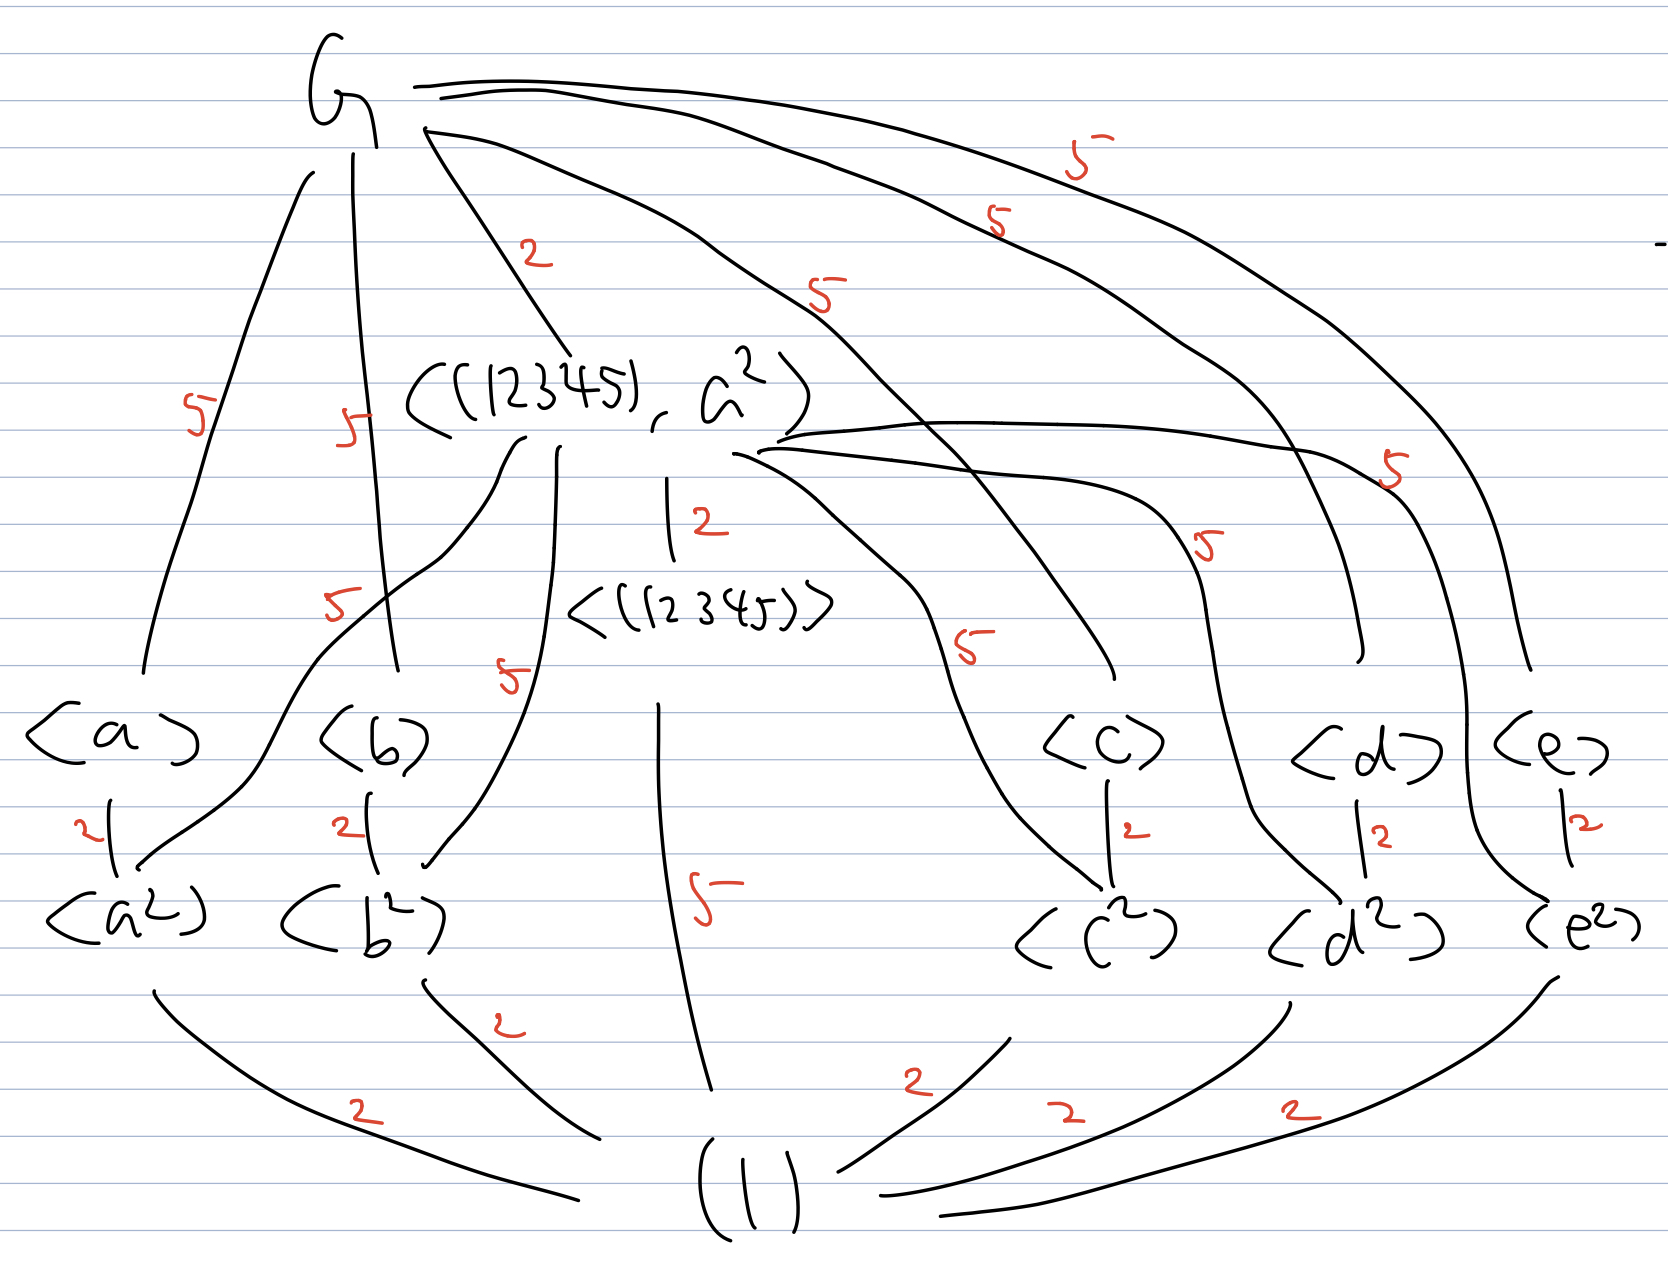
\includegraphics[width=.7\linewidth]{subgroups.jpeg}
    \caption{Subgroups}
    \label{fig:subgroups}
  \end{figure}
  Figure \ref{fig:subgroups} shows all the subgroups of $G$ where $a = (1325), b = (1435), c = (1243), d = (1254), e = (2354)$.
  By the fundamental theorem of Galois theory, there is a bijective correspondence between intermediate groups and intermediate fields, and the inclusion is reversed.
  The degree of extension corresponds to the index.
  By Lagrange's theorem, it is clear that, between any two groups connected by an edge in the figure, there cannot be any proper subgroups between them.

  The number of subgroups of order 4 and 5 must be 5 and 1 by Sylow's theorem.
  By writing out all the 20 elements
  \begin{align*}
    (1),(12)(35),(12345),(1243),(1254),(13)(45),(1325),(1342),(13524),(14)(23), \\
    (14253),(1435),(1452),(15)(24),(1523),(1534),(15432),(2354),(2453),(25)(34),
  \end{align*}
  we conclude that the number of elements of order 2 is 5.
  Thus the number of subgroups of order 2 is 5.
  Finally, $G / \ev{(12345)}$ is isomorphic to $\mathbb{Z}/4$.
  Therefore, there can be only one subgroup of order 10 between $G$ and $\ev{(12345)}$.
  Conversely, since every subgroup of order 10 must contain a subgroup of order 5, $\ev{(12345), a^2}$ is the only subgroup of order 10.

  In order to check which intermediate fields are Galois, it suffices to check normality.
  By the index, $\ev{(12345), a^2}$ is normal in $G$.
  Clearly, $\ev{(1)}$ and $G$ are normal in $G$.
  $\ev{(12345)}$ is normal since it is only subgroup of order 10.
  The other subgroups are not normal.
  For instance, $b\ev{a^2}b^{-1} \ne \ev{a^2}$.
\end{exer}

\end{document}


